\chapter{First Prototype}
The first prototype for the detection of clapping was created with Particle's Photon Board. For this purpose the circuit was rebuilt as shown in Figure \ref{fig:photonBoard}\footnote{Source: MSc\_DCSE\_Assignment\_WS6\_Smartphone\_Sensing\_meets\_IoT\_2018\_final} and a test program was loaded with the corresponding Web IDE with which it is possible to collect initial data.
\begin{figure}[h]
	\centering
	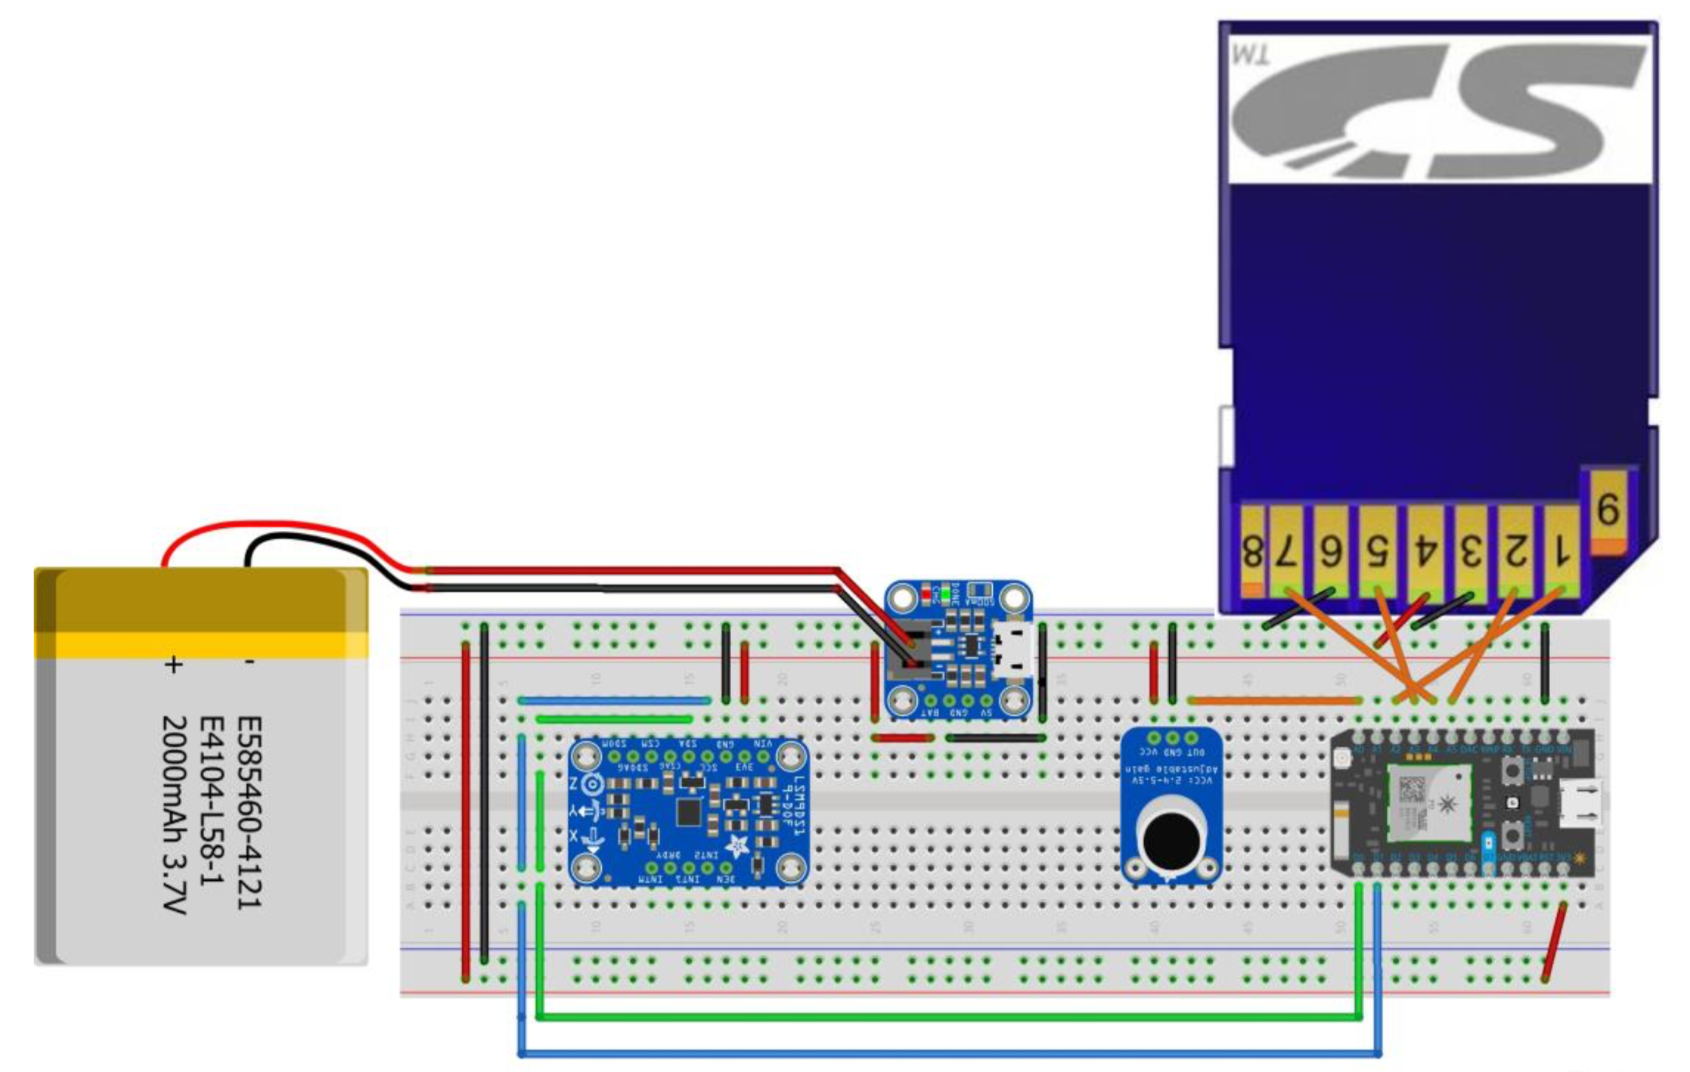
\includegraphics[width=.7\textwidth]{imgs/particleBoard}
	\caption{Particle's Photon Board}
	\label{fig:photonBoard}
\end{figure}
\newpage
The first six measurements were made at a sampling rate of 10Hz. By performing the Fast Fourier transformation on the collected amplitudes, it was possible to examine the amplitude spectrum. Figure \ref{fig:clapping10Hz} shows one result that captured the clapping correctly. This was not the case with every measurement. It can be said that 10Hz is too little for sampling, since possible clapping cannot be measured correctly or only partially in this way. 
\begin{figure}[h]
	\centering
	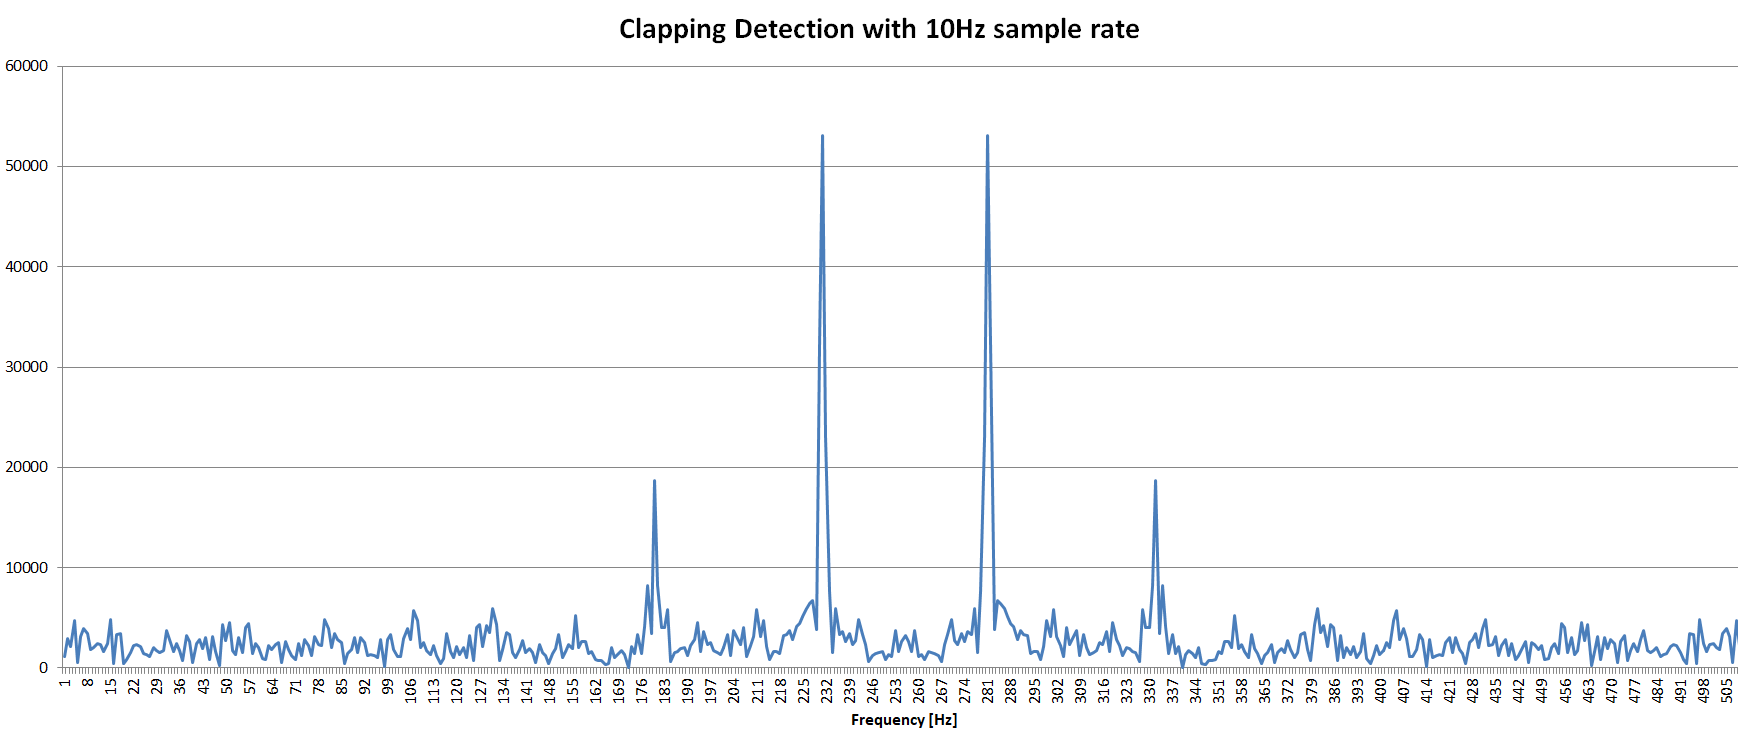
\includegraphics[width=\textwidth]{imgs/clapping10Hz}
	\caption{Amplitude Spectrum for Clapping with 10Hz sample rate}
	\label{fig:clapping10Hz}
\end{figure}
\\
A possible solution is therefore to increase the sampling rate to 1kHz. 
\\\\
The following measurements have shown that writing to the SD card is too slow in each iteration, resulting in a reduced sampling rate of about 200Hz. It is therefore an idea to keep the data in the memory of the board until enough data has been collected to be written to the SD card at once. 
\newpage
By holding the data in the memory of the board, it is possible to obtain a higher sampling rate. However, the evaluation of the data is time-consuming, since they first have to be transferred from the SD card to a PC. With many measurements, the time adds up and makes the measurements no longer efficient. \\
Therefore, it makes more sense to use an Android smartphone with its microphone that can send the created CSV files directly, for example to the dropbox. Thus the data is quickly available for several persons and evaluations can be made directly. The implementation of the software for the Android phone and the used libraries are described in more detail in chapter XYZ!!!!!!!!!!!!!!!!!!!
\section{Measurements with Android phone}
The first measurements with a sample rate of 22kHz generated the following figure (Figure \ref{fig:clappingAndroid}). Compared to Figure \ref{fig:clapping10Hz}, it can be said that the values for the frequency do not match. 
\\\\
\begin{tabular}{|l|l|}
	\hline
	\textbf{Particle} & \textbf{Android} \\
	\hline
	230Hz & 160Hz\\
	\hline
\end{tabular}
\\\\
For this reason, it makes sense to check the generated data of the smartphone and the associated calculations with another tool. This is done using the iSpectrum software, which can be installed on a MacBook. This makes it possible to collect live data from the laptops microphone to view the spectrum. 
\newpage
\begin{figure}[h]
	\centering
	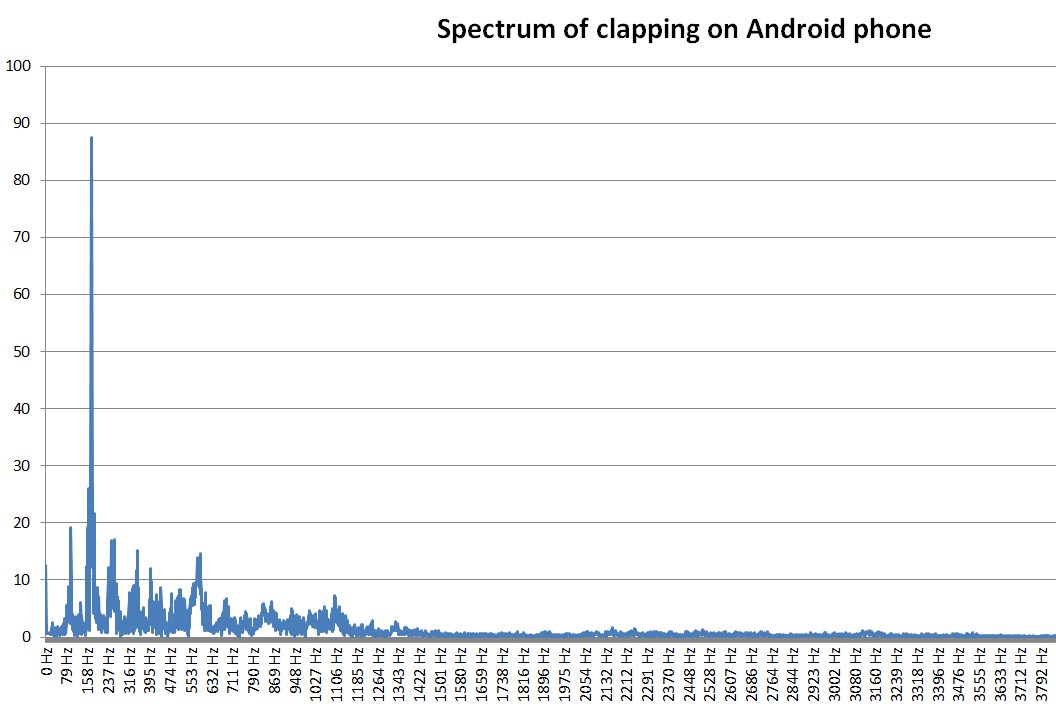
\includegraphics[width=\textwidth]{imgs/clappingAndroid}
	\caption{Amplitude Spectrum for Clapping with Android device}
	\label{fig:clappingAndroid}
\end{figure}
In order to compare the iSpectrum software and the Android device, a reliable source is needed that provides values for a specific frequency. The idea is to take a sound example and play it to both systems. This makes it possible to observe which values are output for the frequency.
\\
Instead of a single sound file, a video is used for testing, which plays all frequencies in the audible range of the human ear. This video is called \textbf{20Hz to 20kHz (Human Audio Spectrum)}\footnote{https://www.youtube.com/watch?v=qNf9nzvnd1k}. It is thus possible to see whether the values are correctly interpreted with different frequencies in the Android device.
It is thus possible to see whether the values are correctly interpreted with different frequencies in the Android device.
\newpage
\begin{figure}[h]
	\centering
	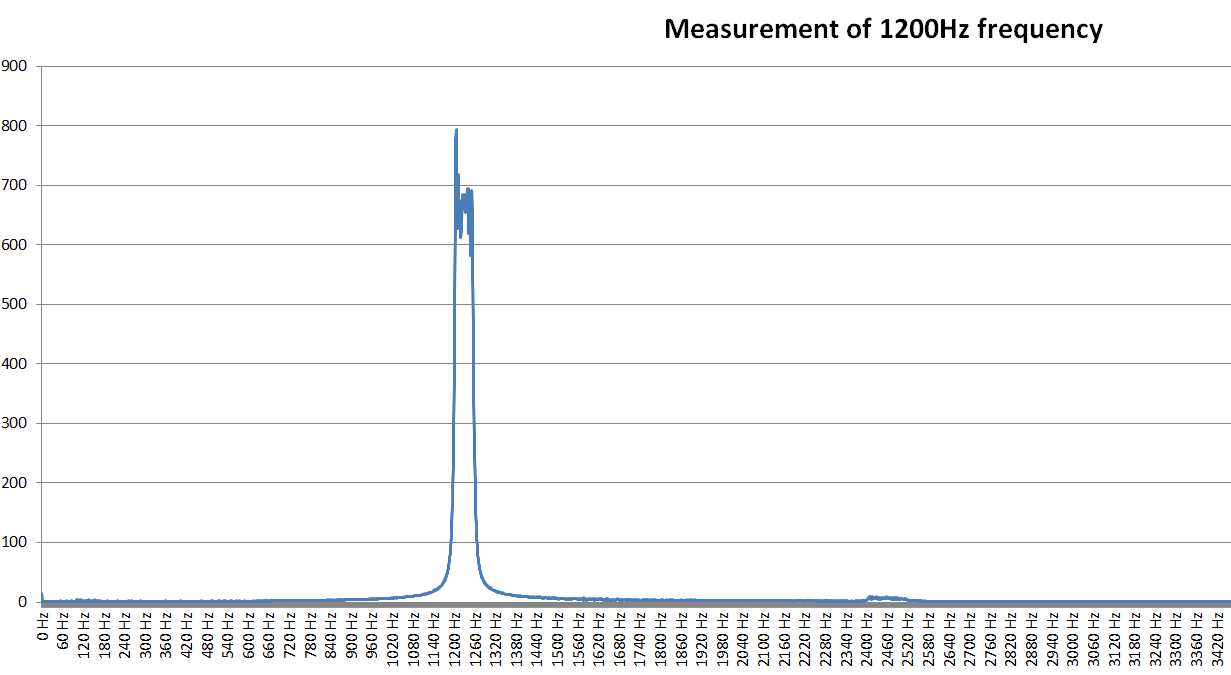
\includegraphics[width=.9\textwidth]{imgs/yt1200Hz}
	\caption{Amplitude Spectrum for 1200Hz (Android device)}
	\label{fig:1200HzAndroid}
\end{figure}

\begin{figure}[b!]
	\centering
	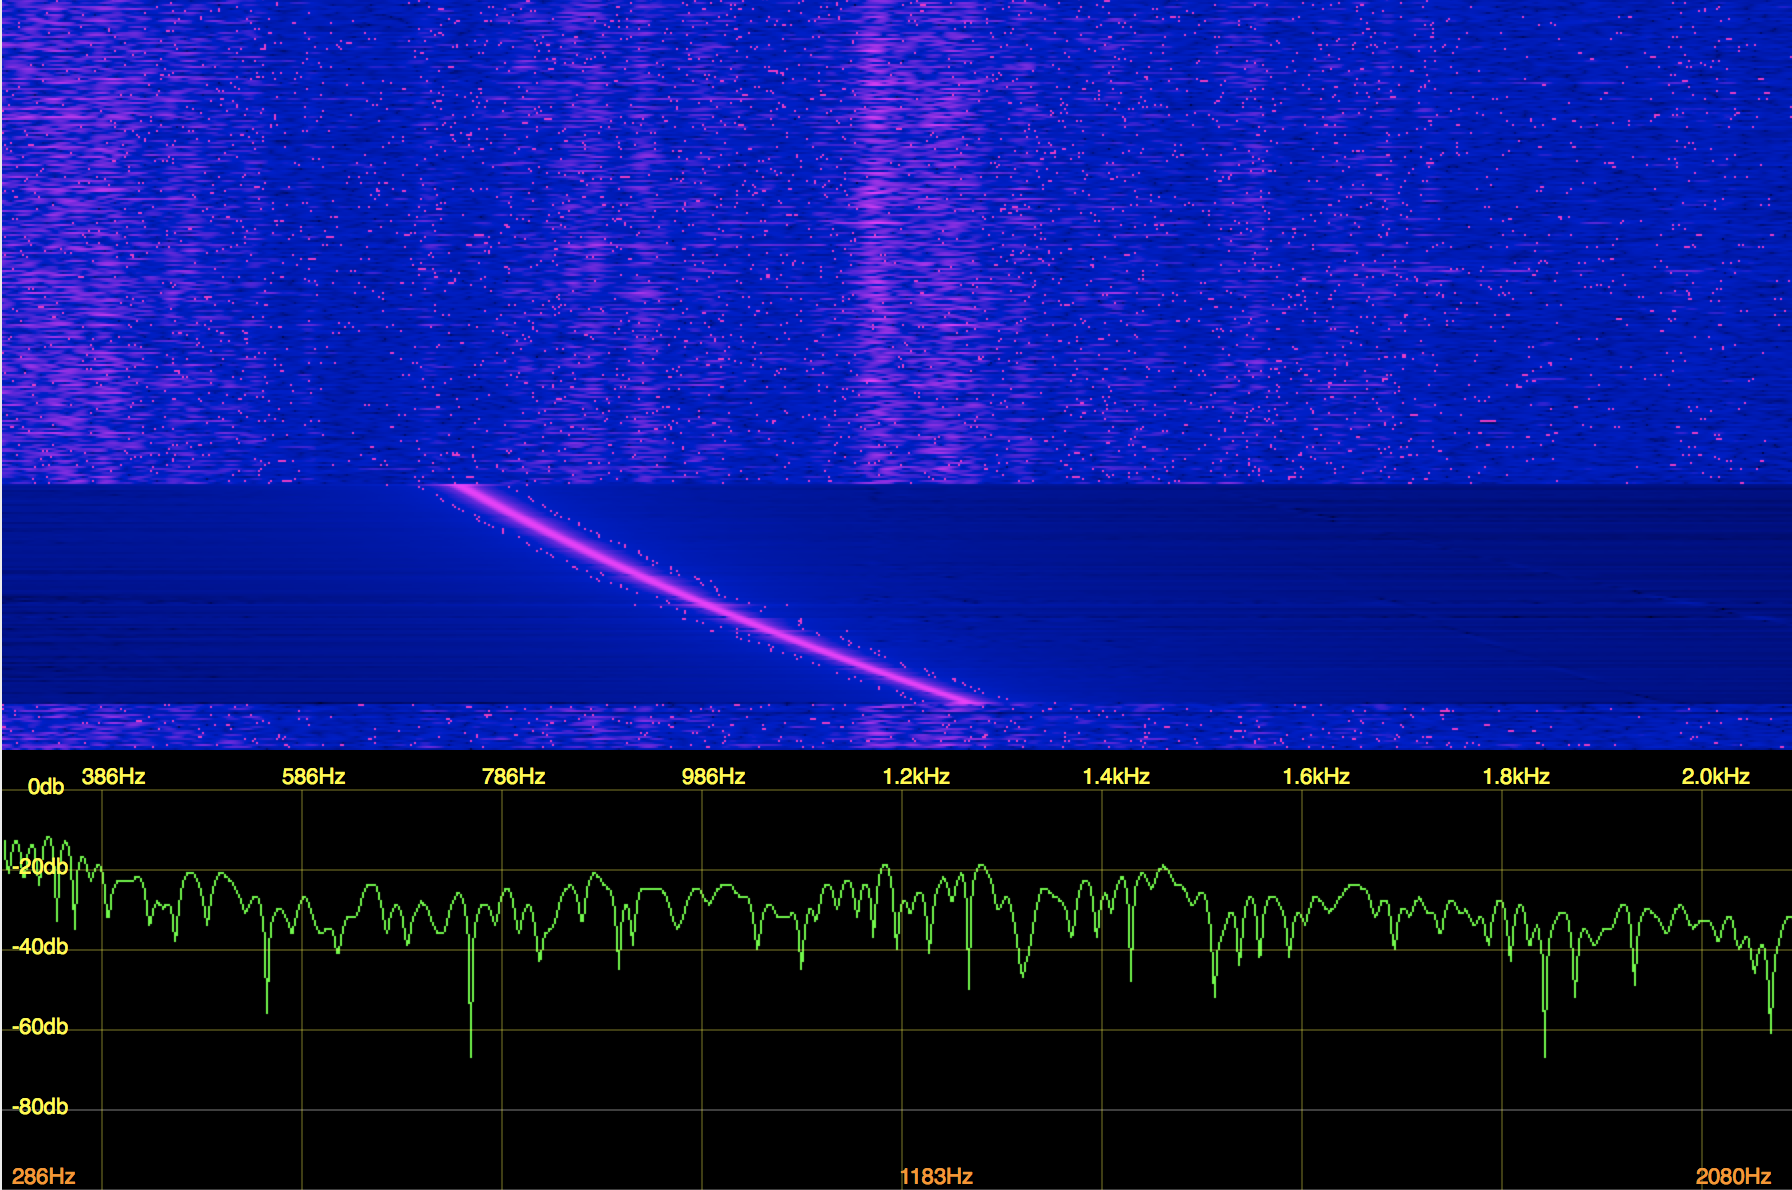
\includegraphics[width=.8\textwidth]{imgs/iSpectrum1200Hz}
	\caption{Amplitude Spectrum for 1200Hz (iSpectrum)}
	\label{fig:1200HziSpectrum}
\end{figure}
\newpage
As figures \ref{fig:1200HzAndroid} and \ref{fig:1200HziSpectrum} show, the 1200Hz are reliably detected by both systems. Live testing with iSpectrum makes it very convenient to make clapping and other noises visible. Therefore, different sounds were tried out to see what the spectrum looks like.
\begin{figure}[h]
	\centering
	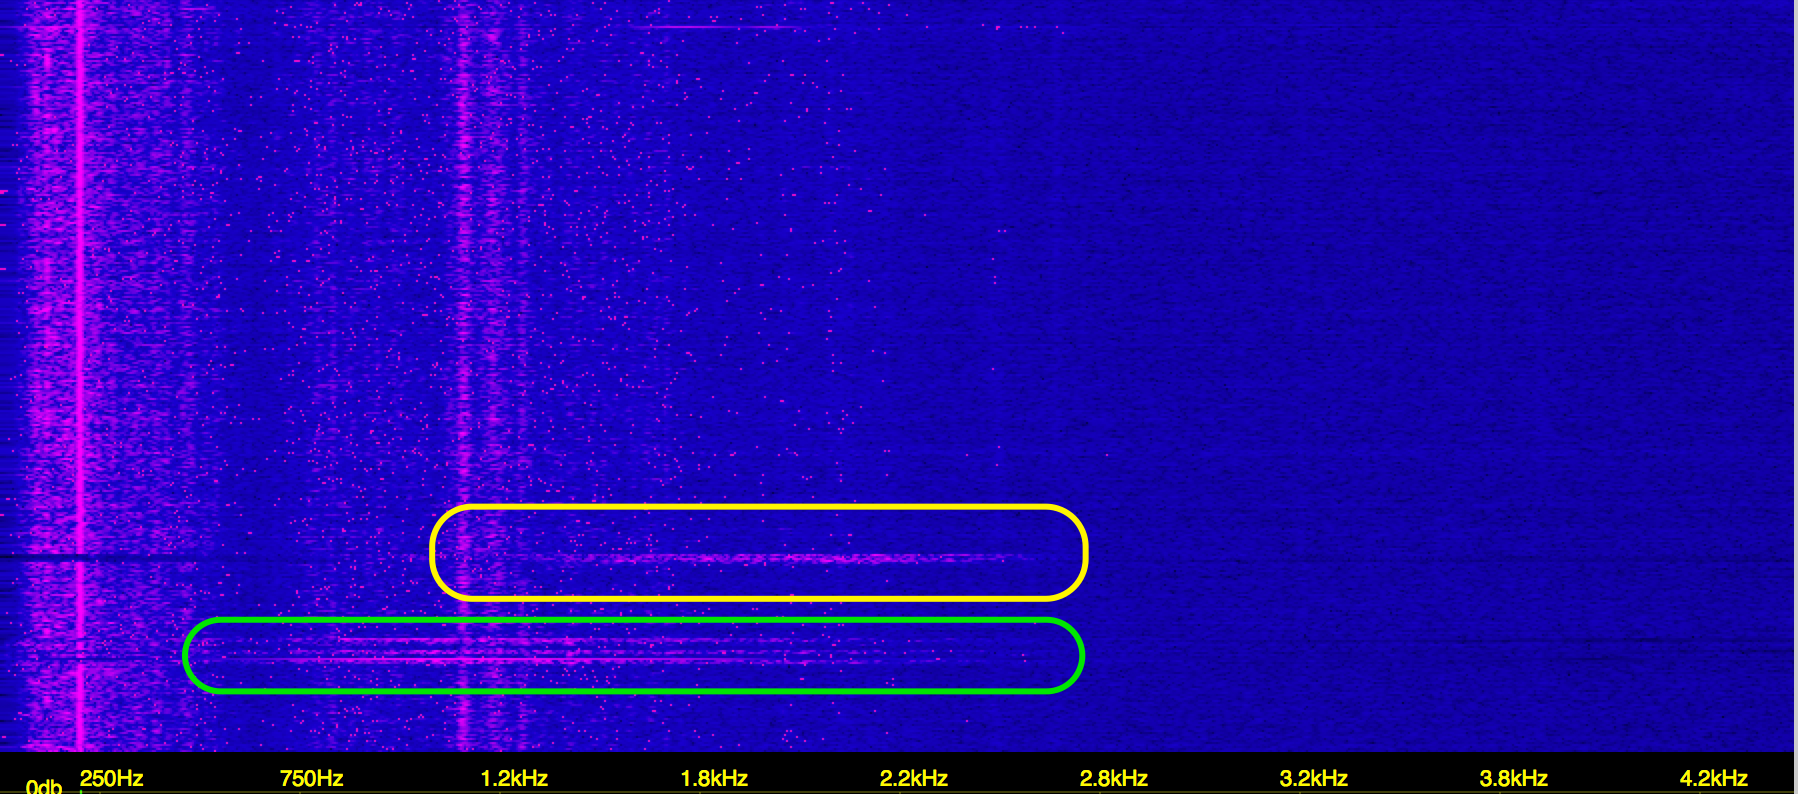
\includegraphics[width=\textwidth, trim={0 0 2cm 5cm},clip]{imgs/iSpectrumClappingKnocking}
	\caption{Spectrum of clapping and knocking}
	\label{fig:clappingKnocking}
\end{figure}\\
The yellow circle in Figure x shows the clapping in a small room. The three sounds detected, which have a green frame, are knocking on the table. It can be seen that these noises occur in different frequency ranges. However, each clapping or tapping can be different from person to person, depending on how much clapping or tapping occurs, or where the person is. Further measurements with various test subjects have shown this. A distinction can possibly be made with the duration of the sound. The clapping echoes a little and the knocking stops abruptly. It probably makes more sense to consider the duration of the clap than the frequency range.
